\documentclass[a4paper, 12pt]{report}
\usepackage[utf8]{inputenc}
\usepackage{graphicx}
\usepackage{xcolor}
\usepackage{appendix}
\usepackage[top=2cm, bottom=2cm, left=2cm, right=2cm]{geometry}
\usepackage[francais]{babel}
\usepackage{hyperref}
\hypersetup{
    colorlinks=true,
    linkcolor=black,
    urlcolor=black,
    linktoc=all
}

\usepackage{fancyhdr}
\usepackage{lastpage}

\addtocontents{toc}{\protect\thispagestyle{fancy}}

\pagestyle{fancy}
\setlength\headheight{12mm}
\fancyhf{}
\lhead{
\includegraphics[height=1cm]{../../public/images/Logo-spf-sm.png}}
\chead{}
\rhead{
\includegraphics[height=8mm]{../../public/images/Logo-entremploi-sm.png}}
\lfoot{\today}
\cfoot{}
\rfoot{page \thepage \ / \pageref{LastPage}}

\title{Entr'Emploi}
\author{MAILLARD Noé MILSONNEAU Jean}

\begin{document}

\begin{titlepage}
	\thispagestyle{empty}
    \centering
    {\bfseries\Large
    		Site internet EntrEmploi\\
        \today\\
        \vskip3cm
        
\includegraphics{../../public/images/Logo-entremploi-md.png}
        \vskip15mm
        
\includegraphics{../../public/images/Logo-spf.png}
        \vskip3cm
        Maillard Noé, Milsonneau Jean\\
    }
    \normalsize
\end{titlepage}

\tableofcontents
\chapter{Le projet Entr'Emploi}
\thispagestyle{fancy}
\section{Entr'Emploi}
Entr'Emploi a pour projet depuis le debut de l'année d'avoir a disposition un site internet qui leurs permettrait d'avoir plus de visibilité
dans ce monde numérisé. Malheureusement, l'association n'a, ni les personnes compétentes pour réaliser le projet, ni l'argent pour faire appel aux services d'une entreprise.
Nous nous sommes donc proposés d’offrir nos capacités pour mettre au jour ce projet, de plus nous y voyions un excellent moyen d’acquérir de l'expérience et de découvrir de nouvelles technologies.
Le projet consiste donc a faire connaître l'association et son action, procurer à l'équipe d'Entr'Emploi un outil de travail simple et efficace.
\section{La mission d'Entr'Emploi}
Entr'Emploi propose un accompagnement personnalisé pour les chercheurs d'emploi plus ou moins éloigné du marché du travail depuis cette année dans la région de Brest.\\
Ils les aident à clarifier leur projet, s'orienter vers des formations et à organiser leur recherche d'emploi.\\
\begin{itemize}
\item élaboration des CV, rédaction des lettres de motivation ;
\item simulation d’entretien d’embauche ;
\item coaching individuel, atelier collectif « Que dit mon image ? » animé par une professionnelle de l’insertion ;
\item recherche active et dynamique des offres d’emploi grâce à une « veille » permanente, notamment sur les sites Internet, et à la réactivité des accompagnants qui permet d’accroître d’autant les chances d’obtenir un entretien ;
\item la combinaison des activités proposées au sein du Secours populaire qui permet de lever des obstacles :atelier d’estime de soi,alimentaire, vestiaire, permanence juridique, bientôt conseiller en budget familial, etc.cours d’informatique et de français pour les étrangers.
\end{itemize}
\ \\
Il s'agit de renforcer et de compléter les services proposés par les organismes existants, en apportant aux chômeurs un soutien supplémentaire, structuré et sur le long terme si nécessaire.\\
Ce projet date de 2015 et est mis en place à Brest et également à Quimper, il est très probable que le projet inspire d'autres régions à mettre en place le même programme d'aide.\\
Pour cela ils proposent différentes prestations d’accompagnement :


\chapter{Analyse de l’opération}
\thispagestyle{fancy}
\section{Pourquoi un site internet web ?}
Le projet Entr'Emploi est un projet relativement récent, encore de sa phase de construction. il faut donc le faire
connaître au monde, et ce de la manière la plus efficace qui soit. La réponse est simple : un site internet.
c'est accessible en permanence depuis n'importe quel endroit dans le monde, et cela permet une expansion vers d'autres
régions de la France si le projet se montre concluant.
\section{Fonctionnalités du site}
Le site internet doit permettre aux demandeurs d'emploi de trouver une panoplie d'offres d'emplois et surtout de faire
appel aux services proposés par Entr'Emploi (Ateliers CV, estime de soi, simulation d'entretien).
les entreprises, quant à elles, peuvent faire publier leurs offres d'emploi par les bénévoles sur le site et également
parcourir une CV-thèque pour trouver le profil qui correspond le mieux a leur demande.\\
voici la liste des fonctionnalités issue de notre seconde réunion (A.4):
\begin{itemize}
    \item Présentation du projet
    \item Prestation
    \item CVthèque
    \item Offres d'emploi
    \item Liste de partenaires
    \item Lien vers la fédération/don/bénévolat
\end{itemize}
Pour les bénévoles, une page d'administration sera disponible pour leur permettre d'éditer les offres et C.Vs.

\chapter{Calendrier prévisionnel}
\thispagestyle{fancy}
\section{Date importantes}
\begin{itemize}
\item Première rencontre (8/10/15 A.3)
\item Présentation de la maquette (19/11/15 A.5)
\item Présentation du prototype (janvier 2016)
\item Validation du prototype (fin mars 2016)
\item Mise en ligne (début avril 2016)
\item Soutenance (19/05/16)
\end{itemize}
Pour une vue en détail de l'organisation du planning le diagramme de Gantt est disponible en annexes
\section{Réunions}
Les réunions avec l'équipe de bénévoles sont des moments important pour nous permettre d'écouter les retours de l'équipe sur notre travail, c'est pourquoi nous avons prévu de nous voir régulièrement. Les comptes rendu des trois réunions déjà effectué sont disponible en annexe.\\ Les dates des réunions suivantes restent a déterminer en fonction des emplois du temps de chacun mais nous avons prévu au minimum de nous revoir en janvier puis trois autres fois autour de la mise en ligne du site affin d'assurer un début efficace au site.

\chapter{Résultats envisagés}
\thispagestyle{fancy}

\section{Objectif visé}
L'objectif du projet est de livrer un site simple et facile d'utilisation, réalisé en collaboration étroite avec l'équipe d'Entr'Emploi.
En parallèle du site internet, Nous nous sommes fixé comme objectif de créer un plateforme sur laquelle il est possible d'éditer
le site internet lui-même sans avoir besoin de modifier le code source du projet. L'extensibilité aux instances du secours populaire en France
est aussi un aspect important du site internet.

\section{Outils de mesure}
Après avoir mis le site en ligne, transmis a l'équipe d'Entr'Emploi tous les documents leurs permettant de bien utiliser leur nouvel outil de travail, il faut pouvoir vérifier si nos efforts
ont conduits a un succès ou à un échec. Voici les différentes moyen que nous aurons a disposition pour mesurer les résultats :
\begin{itemize}
    \item En consultant le site de manière régulière, nous pouvons voir si il est mis a jour, donc utilisé.
    \item Nous aurons aussi accès au statistiques de visites du site, ce qui est un bon facteur quantitatif des résultats.
    \item Si nous n'avons pas a faire d'interventions parce que quelque chose ne fonctionne pas.
\end{itemize}

\chapter{Nos outils de travail}

Notre passion pour l'informatique nous a poussée a utiliser les dernières technologies en matière de développement
web.
Le site web est donc divisé en deux grandes parties :
\begin{itemize}
    \item La partie serveur :
    \begin{itemize}
        \item Node.js pour le serveur à proprement parler
        \item MongoDB pour les bases de données
    \end{itemize}
    \item La partie client :
    \begin{itemize}
        \item HTML5/CSS3 pour la structure et la pise en page.
        \item AngularJS pour l'interaction avec le serveur.
    \end{itemize}
\end{itemize}

Travailler a plusieurs sur un projet pose des problèmes au niveau de la synchronisation, nous utilisons
donc git, un système de contrôle de version, qui nous laisse contribuer au projet chacun de notre côté tout
en permettant de documenter la progression de notre projet.

\newpage
\appendix
\chapter{}
\thispagestyle{fancy}
\section{Charte Graphique}
La charte graphique de notre projet est un élément centrale de notre travail qui évolue avec le reste du projet. On peut tout de même aujourd'hui fixer certaines règles que nous devrons respecter. Nous avons fait le choix de coller au logo actuel du secours populaire.\\
\\
\begin{tabular}{ c  p{10cm}  p{6cm}  }
\raisebox{-\totalheight}{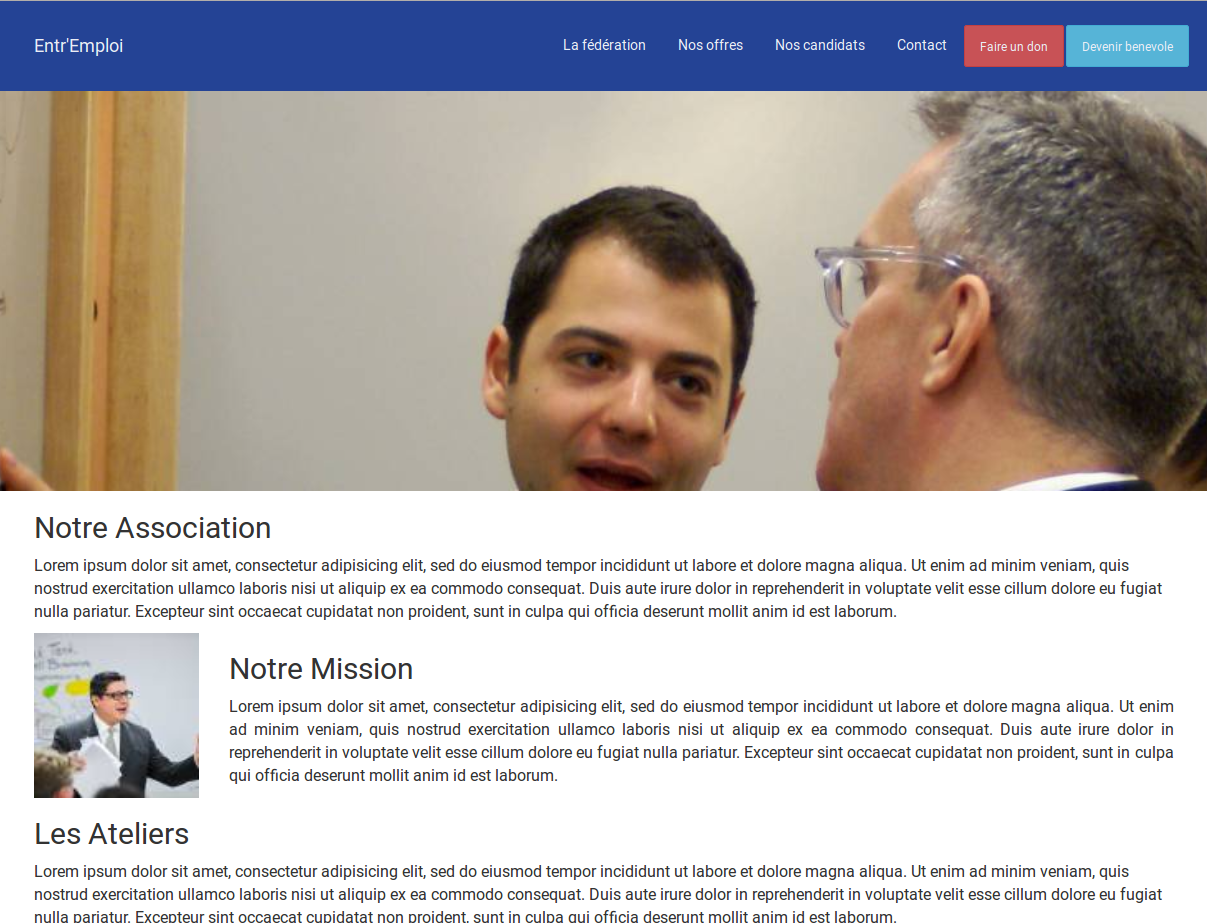
\includegraphics[width=6cm]{maquette1.png}}
&
Notre charte graphique est donc sobre, principalement composé de bleu, blanc et rouge. le bleu étant utilisé pour les menus alors que le rouge trouve sa place pour les boutons et informations importantes. Le visuel ci-contre provient de la première maquette qui va évoluer pour, notamment, se rapprocher plus du visuel du site du secours populaire (Cf A.5).\\
\end{tabular}

\section{Diagramme de Gantt}
\begin{center}
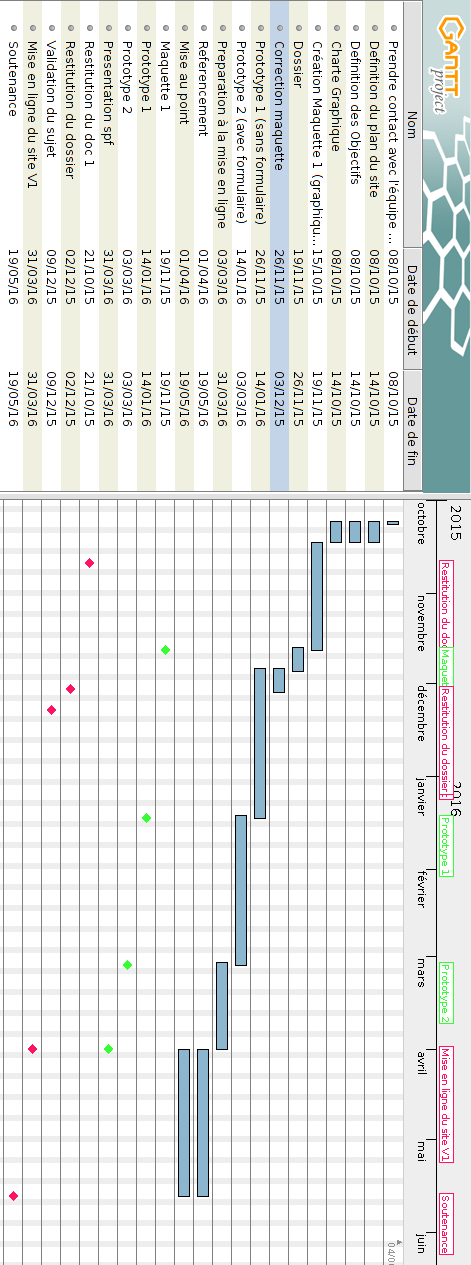
\includegraphics[height=24cm]{gantt.png}
\end{center}
\newpage
\section{Première Réunion - 8/10/15}
La première réunion en présence de Mr Redou nous a permis de prendre conscience de l'envergure du travail a fournir. Nous avons alors constaté qu'il était nécessaire de créer complètement le site. Après discutions nous avons décidé de concentrer notre projet uniquement autour de la création du site dans le but d’être certain de pouvoir fournir le meilleur outil possible.
\section{Seconde Réunion - 15/10/15}
Notre seconde réunion en présence d'une partie de l'équipe d'EntrEmploi nous a permis de nous présenter de mettre a plat le besoin auquel nous pouvons tenter de répondre avec nos ressources. Nous nous sommes mis d'accord sur les objectifs et fonctionnalités à fournir suivantes:\\
Objectifs:
\begin{itemize}
    \item Faire connaître Entr'Emploi
    \item Donner envie à des chercheurs d'emploi de faire appel a Entr'Emploi
    \item Donner envie aux recruteurs d'utiliser le site
    \item Faire connaître la fédération
\end{itemize}
Fonctionnalités:
\begin{itemize}
    \item Présentation du projet
    \item Prestation
    \item CVthèque
    \item Offres d'emploi
    \item Liste de partenaires
    \item Lien vers la fédération/don/bénévolat
\end{itemize}
Nous avons également choisi de reprendre le code couleur du logo du secours populaire pour la charte graphique en nous basant également sur le site du secours populaire.
\section{Troisième Réunion - 19/11/15}
En présence d'une plus grande partie de l'équipe nous avons présenté une maquette du site dans le but de clarifier les attentes de l'équipe envers le site. Nous avons également rencontré le bénévole qui sera responsable de la mise à jour du contenu du site.\\
Nous avons également discuté de la présence des différents logos et de l'importance que le site soit clairement en lien avec le secours populaire, en particulier la présence de redirections vers les pages de dons et de bénévolat du secours populaire.\\
Pour finir, après avoir écouté différentes suggestions et inquiétude de l'équipe nous nous sommes mis d'accord sur une liste de changement à effectuer sur la maquette et sur notre planning qui prévoit une autre réunion en janvier.\\
Une réflexion sur le nom de domaine doit encore être faite autour de ses différents noms de domaines:
\begin{itemize}
    \item www.entremploi.org
    \item www.entremploi29.org
    \item www.entremploi26.bzh (coût élevé)
    \item www.entremploi.secourspopulaire.fr
    \item www.entremploi.spf29.org
\end{itemize}
\end{document}
